\section{\secondtitle}

\def\secondtitleF{Predicting learned-cuts}
\def\secondtitleS{Applying learned-cuts to the MFMP}


\begin{frame}
\frametitle{\textbf{Contents}}
  \setbeamercovered{transparent}
  \begin{block}{\textbf{\secondtitleF}}
  \end{block}  

  \only<1>{
    \begin{block}{\textbf{\secondtitleS}}
    \end{block}  
  }
  \only<2->{
    \transparent{0.3}
    \begin{block}{\textbf{\secondtitleS}}
    \end{block}  
    \transparent{1}
  }

\end{frame}

\begin{frame}[t]
\frametitle{\textbf{Predicting learned-cuts}}
  \pause
  \begin{tabular}{ll}
  \onslide<+->{
    \textbf{Optimization problem} & $y^{*}(x) :\equiv arg \,\,\min_{y \in \mathcal{Y}(x)} C(x,y)$
    } \\
  \onslide<+->{
      \textbf{Solution features} & $G(y) = \{g_n(y) \,\, \forall n \in \mathcal{N}\}$
  } \\
  \onslide<+->{
      \textbf{Input features} & $H(x) = \{h_m(x) \,\, \forall m \in \mathcal{M}\}$ 
  }\\ 
  \onslide<6->{
      \textbf{Training for optimal} & $G(y^*(x)) \approx \hat{G}(x) = f(H(x)) \, \star$
  } \\
  \end{tabular}

  \only<2>{
   \begin{adjustbox}{max totalsize={.5\textwidth}{.5\textheight},center}
      \DrawSolution{none}{none}{0}
   \end{adjustbox}
  }
  \only<3-4>{
   \begin{adjustbox}{max totalsize={.5\textwidth}{.5\textheight},center}
      \DrawSolution{gy}{none}{0}
   \end{adjustbox}
  }
  \only<5->{
   \begin{adjustbox}{max totalsize={.5\textwidth}{.5\textheight},center}
      \DrawSolution{gyoptim}{none}{0}
   \end{adjustbox}
  }
  \begin{textblock*}{1.1\textwidth}(0.8cm, 8cm)
    \begin{flushleft}
    % $\star$
    \onslide<6->{
      \citesize $\star$ E. Larsen, S. Lachapelle, Y. Bengio, E. Frejinger, S. Lacoste-Julien, and A. Lodi. Predicting Tactical Solutions to Operational Planning Problems under Imperfect Information. arXiv, 2018.
    }
    \end{flushleft}
  \end{textblock*}

\end{frame}

\begin{frame}[t]
\frametitle{\textbf{Applying learned-cuts}}

  \begin{tabular}{ll}
  \onslide<2->{
    \textbf{We predict the optimal features} & $\hat{G}(x) = \hat{g}_n(x) \,\, \forall n \in \mathcal{N}$
    } \\
  \onslide<3->{
      \textbf{We predict the optimal ``zone''} & $\mathcal{Y}^\prime(x) = \{y \in \mathcal{Y} \mid  \hat{G}(x) = G(y) \}$
  } \\
  \onslide<4->{
      \textbf{We solve the predicted model} & $\hat{y}^{*}(x) :\equiv arg \,\,\min_{y \in \mathcal{Y}^\prime(x)} C(x,y)$ 
  }\\ 
  \onslide<5->{
      \textbf{With some (hopefully small) loss} & $C(x,\hat{y}^{*}(x)) \approx  C(x,y^{*}(x))$
  } \\
  \end{tabular}

  \only<1>{
   \begin{adjustbox}{max totalsize={.5\textwidth}{.5\textheight},center}
      \DrawSolution{none}{none}{0}
   \end{adjustbox}
  }
  \only<2>{
   \begin{adjustbox}{max totalsize={.5\textwidth}{.5\textheight},center}
      \DrawSolution{ghat}{none}{0}
   \end{adjustbox}
  }
  \only<3>{
   \begin{adjustbox}{max totalsize={.5\textwidth}{.5\textheight},center}
      \DrawSolution{ghat}{north west lines}{0}
   \end{adjustbox}
   }
  \only<4>{
   \begin{adjustbox}{max totalsize={.5\textwidth}{.5\textheight},center}
      \DrawSolution{ghat}{north west lines}{1}
   \end{adjustbox}
   }
  \onslide<5->{
   \begin{adjustbox}{max totalsize={.5\textwidth}{.5\textheight},center}
      \DrawSolution{ghat}{north west lines}{2}
   \end{adjustbox}
   }
\end{frame}

\begin{frame}
\frametitle{\textbf{Motivation}}

  \pause
  \begin{enumerate}[<+->]
  \item
    \textbf{Performance}: a smaller model is easier to solve.
  \item
    \textbf{User feedback}: direct feedback about the solution without
    needing to solve any model.
  \end{enumerate}
\end{frame}

\begin{frame}
\frametitle{\textbf{Contents}}
  \setbeamercovered{transparent}
  \transparent{0.3}
  \begin{block}{\textbf{\secondtitleF}}
  \end{block}  
  \transparent{1}

  \begin{block}{\textbf{\secondtitleS}}
  \end{block}  
\end{frame}


\begin{frame}[t]
\frametitle{\textbf{New formulation}}
 
  \begin{tabular}{ll}
    \onslide<2->{$a_{ijtt'}$ & : aircraft $i$ is in mission $j$ between $t$ and $t'$.}  \\
    \onslide<3->{$m_{ip}$ &: aircraft $i$ uses check pattern $p$.} \\
  \end{tabular}

  \onslide<5->{
    \begin{align*}
      & \sum_{(j, t, t') \in \mathcal{J}\mathcal{T}\mathcal{T}_{ic}} a_{ijtt'} H^\prime_{jtt'} + U^{\prime}_{tc} \onslide<6-> {\leq H^{M} + bigM (1 - m_{ip})} & \\
      & \hspace{200px}  i \in \mathcal{I}, p \in \mathcal{P}, c \in \mathcal{C}_p
    \end{align*}
  }

  \only<1>{
    \DrawGantt{0}{0}{0}
  }
  \only<2>{
    % missions
    \DrawGantt{0}{1}{0}
  }
  \only<3>{
    % maintenances and missions
    \DrawGantt{2}{1}{0}
  }
  \only<4->{
    % maints, missions and cycles
    \DrawGantt{2}{1}{cycle}
  }
\end{frame}

\begin{frame}
\frametitle{\textbf{Solution features: G(y)}}

  \onslide<+->{
    \DrawGantt{2}{0}{distance}
  }
  \onslide<+->{
    For each aircraft $i$: $D_i(y) \in [E^{min},E^{max}] \,\, \forall y \in \mathcal{Y}(x)$.
  }
  \onslide<+->{
  \begin{block}{\textbf{Average distance between maintenances}}
    $g_1(y) = \mu_{D} = \frac {\sum_{i \in \mathcal{I}} D_i(y)}{I}$. \\
  \end{block}
  }

\end{frame}

\begin{frame}
\frametitle{\textbf{Input features: H(x)}}

  \onslide<1->{  
    \begin{block}{\textbf{Mission related}}
      Max, average, variance of flight hours per period. Median period.
    \end{block}
  }
  \onslide<2->{  
    \begin{block}{\textbf{Fleet related}}
      Sum of initial status (rft).
    \end{block}
  }
  \onslide<3->{  
    \begin{block}{\textbf{Compatibility related}}
      Sum of all special mission flight hours.
    \end{block}
  }
\end{frame}

\begin{frame}
\frametitle{\textbf{Forecasting technique}}

  \onslide<1->{  
    \begin{block}{\textbf{Quantile regressions}}
      Upper bound and lower bound at 10\% and 90\%.
      \begin{equation*}
        \mu_{D} \to [\hat{\mu}_{D}^{lb}, \hat{\mu}_{D}^{ub}]
     \end{equation*}
    \end{block}
  }
  \onslide<2->{  
  \begin{block}{\textbf{Training / test set}}
    of 5000 small instances solved to optimal and splitted: 70/30.
  \end{block}
  }

\end{frame}

\begin{frame}
\frametitle{\textbf{Applying learned-cuts}}

  \begin{block}{\textbf{Pattern filtering:}}
    \begin{equation*}
      D_{ip} \in [\hat{\mu}_{D}^{lb} - tol, \hat{\mu}_{D}^{ub} + tol] \rightarrow p \in \mathcal{P}_i 
    \end{equation*}
  \end{block}
  \pause

  \begin{block}{\textbf{Pattern recycling:} with probabiliy $\alpha$}
    \begin{equation*}
      D_{ip} \notin [\hat{\mu}_{D}^{lb} - tol, \hat{\mu}_{D}^{ub} + tol] \land P(\alpha)  \rightarrow p \in \mathcal{P}_i 
    \end{equation*}
  \end{block}
\end{frame}

\begin{frame}
\frametitle{\textbf{Experiments}}
  
  \begin{itemize}
  \item Number of instances: medium (1000), large (1000) and very large
    (1000).
  \item We seeded instance generation for better comparison.
  \item CPLEX running 1 thread and limited to 1 hour.
  \end{itemize}

  Largest instances have 60 aircraft, 90 periods.
\end{frame}

\begin{frame}[t]
\frametitle{\textbf{Results: performance}}

  \begin{itemize}[<+->]
    \item More solutions.
    \item Faster solutions.
  \end{itemize}

  \only<1>{
    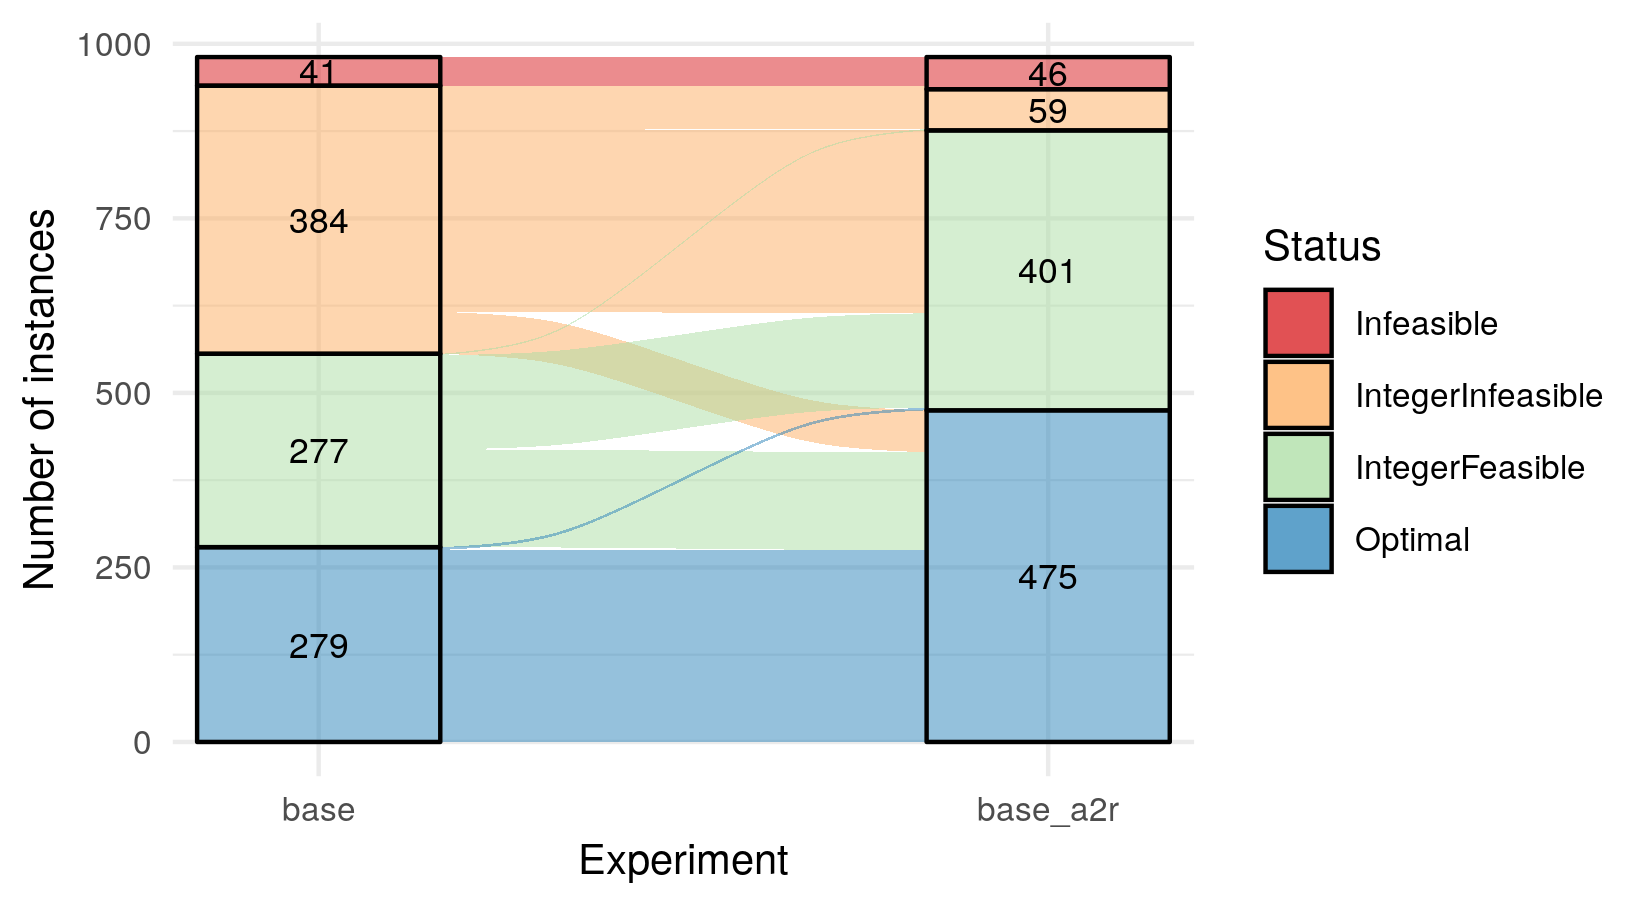
\includegraphics[width=\linewidth]{images/transitions_base_2tasks.png}
  }
  \only<2>{
    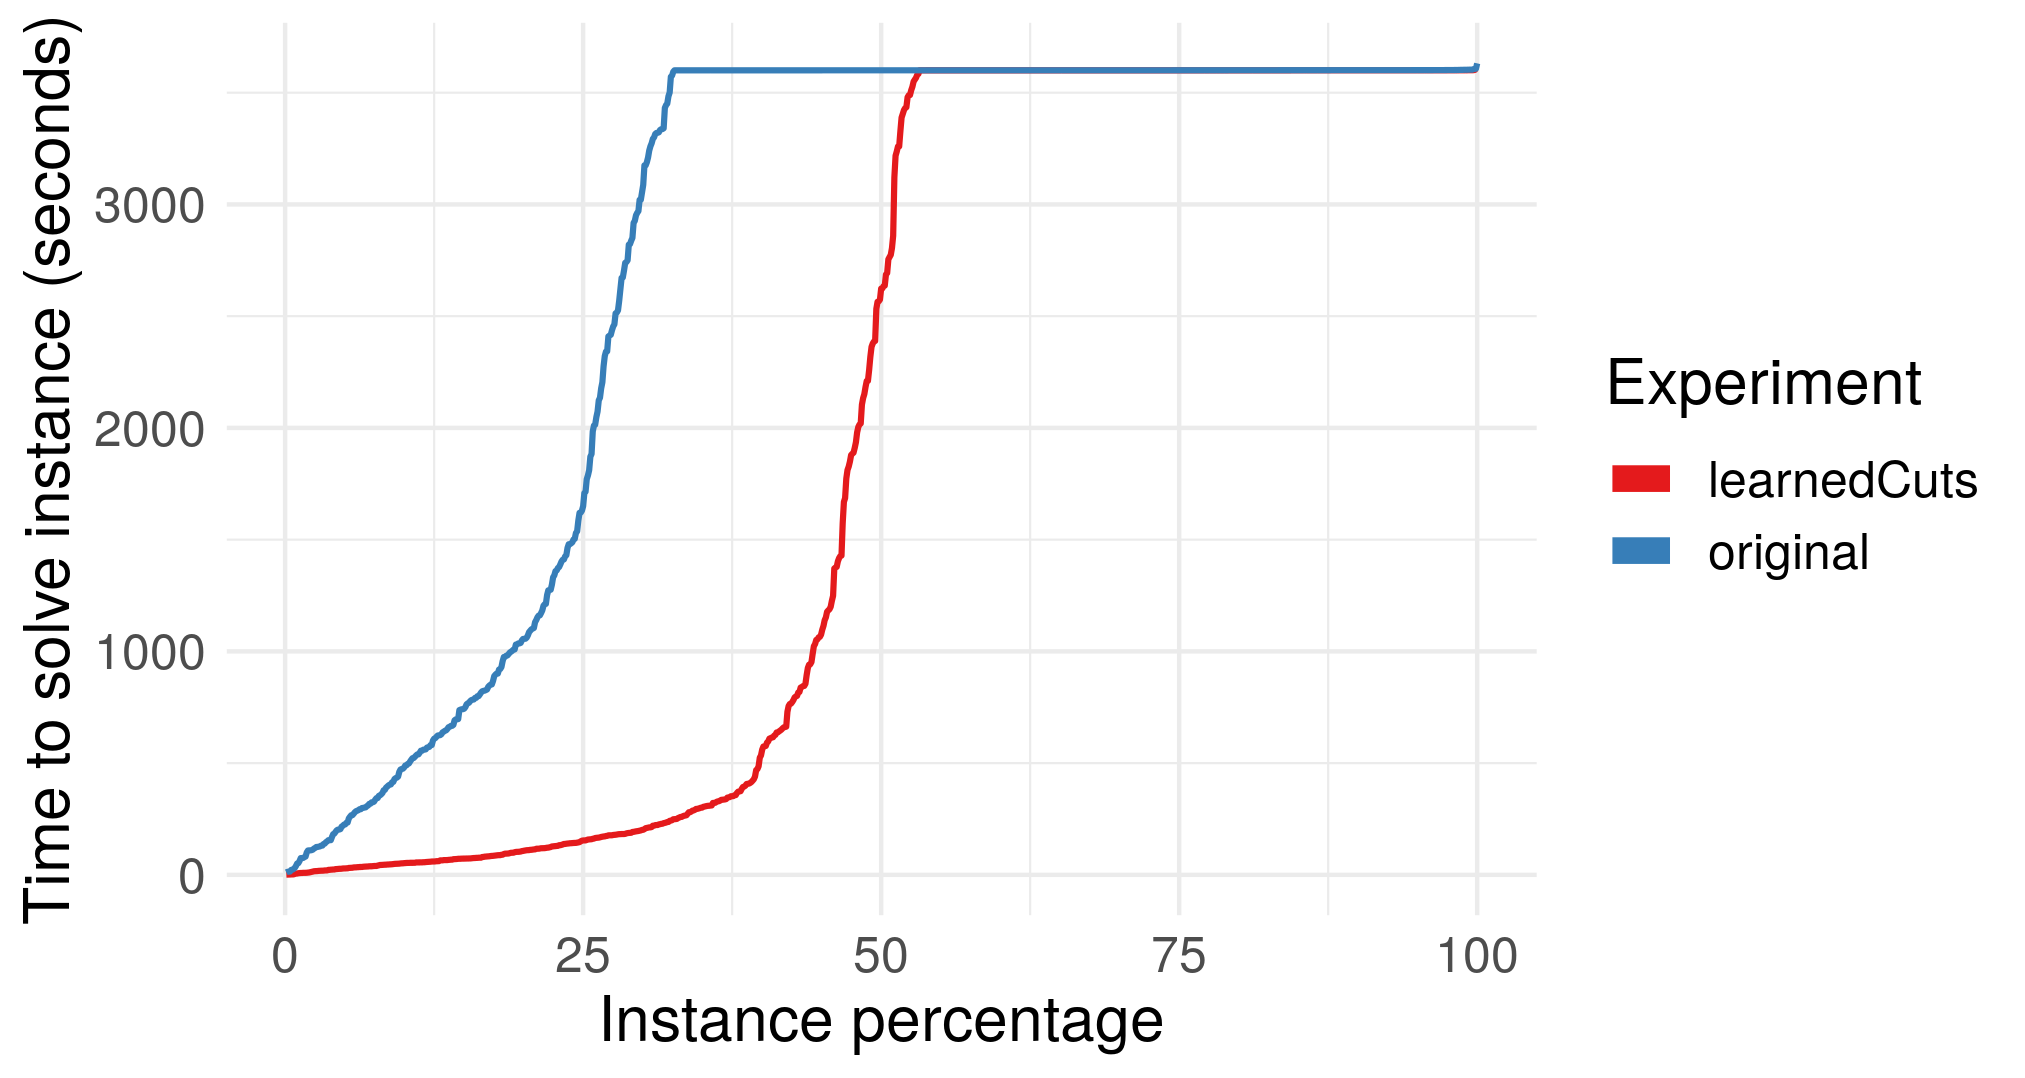
\includegraphics[width=0.8\linewidth]{images/time_performance_ordered_2tasks.png}
  }
\end{frame}

\begin{frame}
\frametitle{\textbf{Results: optimality}}
  
  \begin{itemize}[<+->]
    \item We compare the instances where the two models returned status "optimal".
    \item A reduction of 82.1\% in solution time for these instances.
    \item Less than 7\% loss of optimality for $\ge$ 95\% of these instances. Most below 4\%.
    \item Better predictions can reduce this loss even further.
  \end{itemize}

  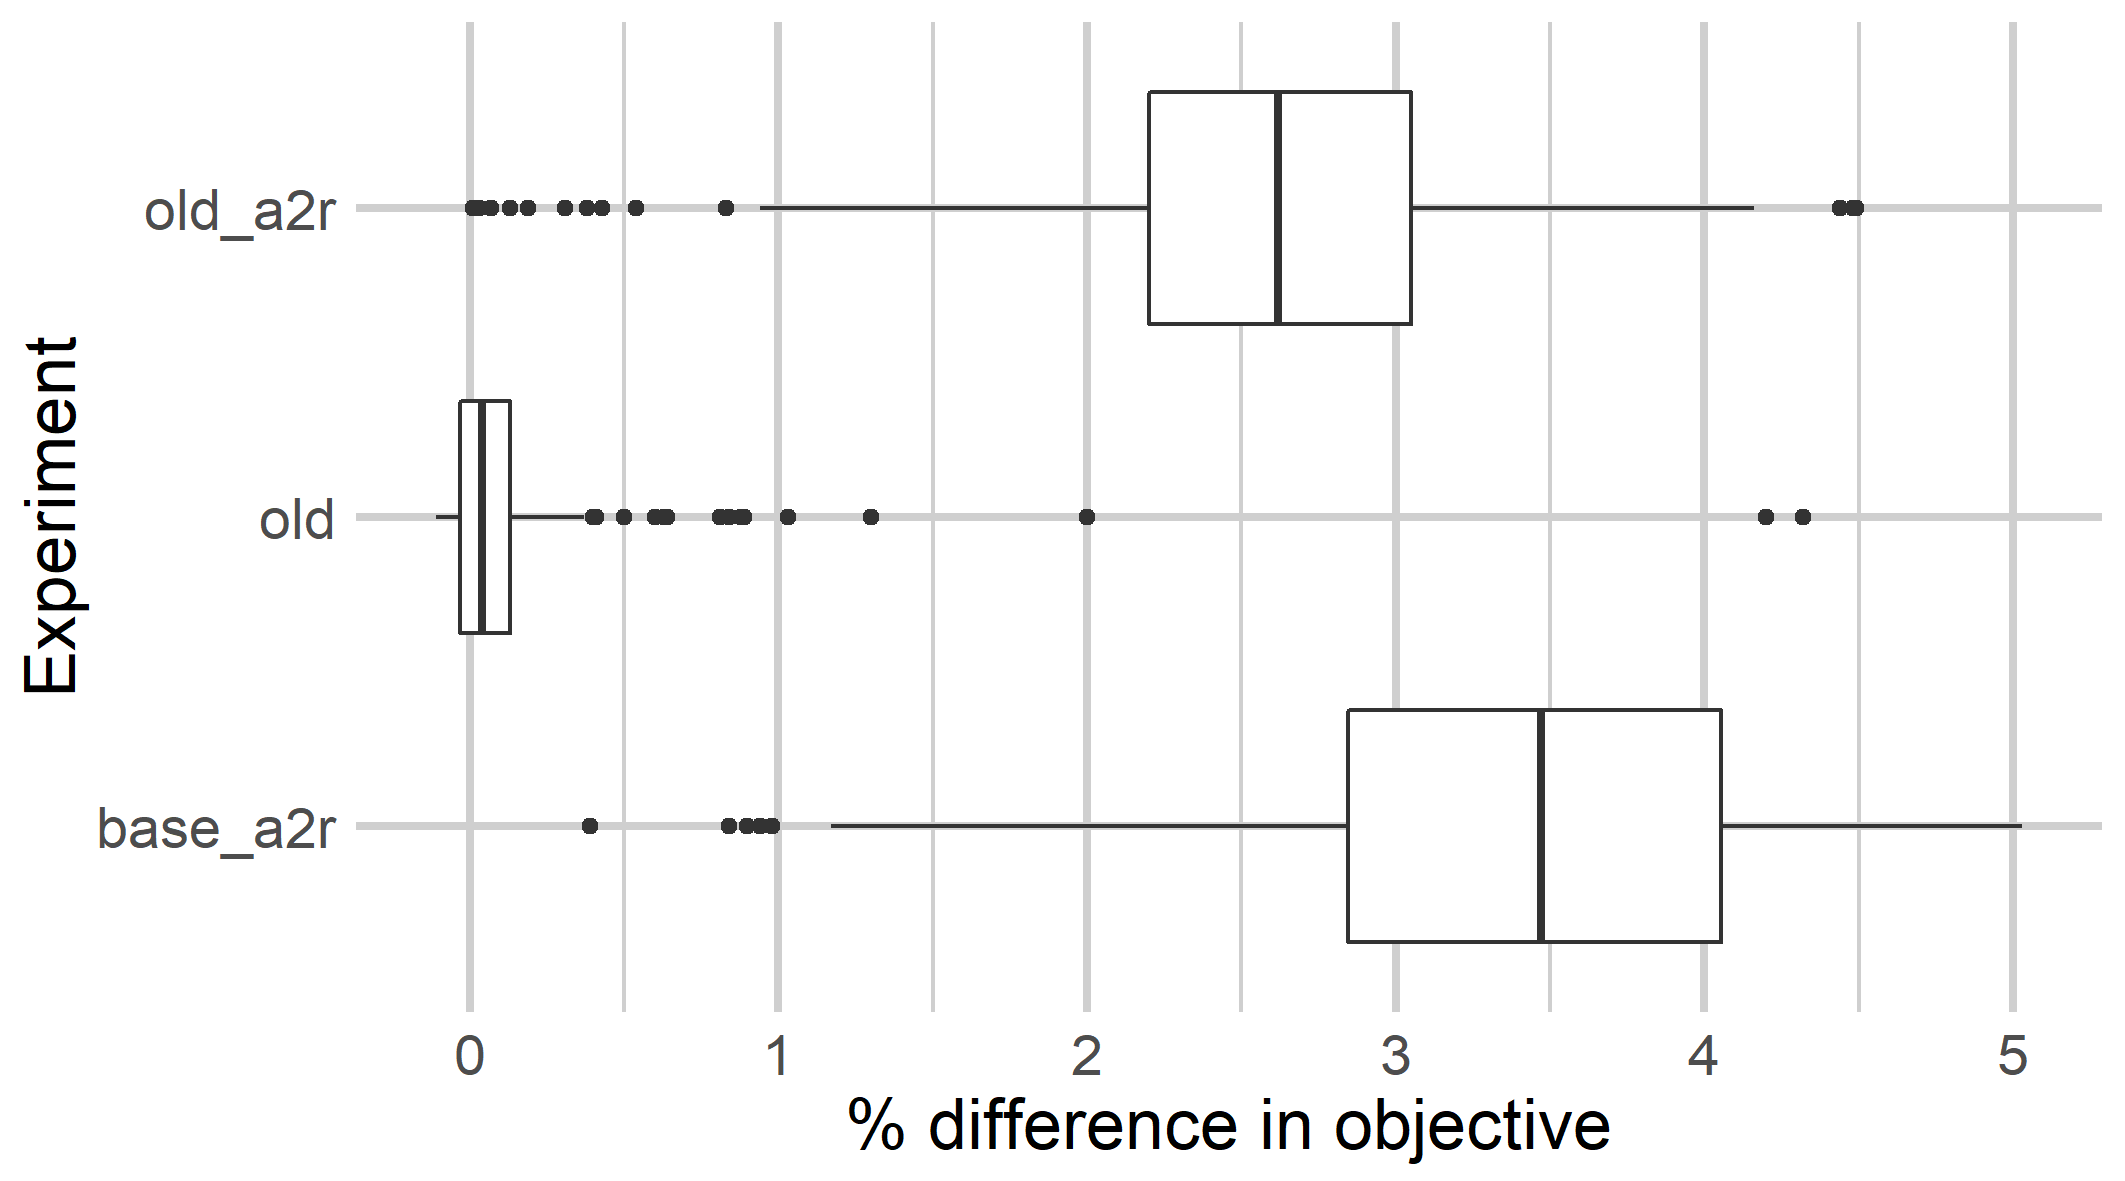
\includegraphics[width=0.8\linewidth]{images/quality_degradation_2tasks}

\end{frame}

\begin{frame}
\frametitle{\textbf{Preliminary conclusions}}
  \pause
  % \begin{block}{}
    \begin{itemize}[<+->]
    \item \textbf{Supervised learning for optimization}
      provides good heuristic solutions.
    \item \textbf{MFMP application}
      shows the benefits of such an approach.
    \end{itemize}
  % \end{block}  
  % \pause
  % \begin{block}{\textbf{Perspectives}}
  %   \begin{itemize}
  %     \item \textbf{Generalize methodology}
  %       to obtain a probability distribution for patterns, automatize feature extraction.
  %     \item \textbf{Combine it with other techniques}
  %       such as Column Generation or graph-based dynamic pattern generation.
  %   \end{itemize}
  % \end{block}  
  \pause
  \textbf{Publication:} Peschiera, F., Dell, R., Royset, J. et al. A novel solution approach with ML-based pseudo-cuts for the Flight and Maintenance Planning problem. OR Spectrum, 2020.
\end{frame}